\section{Test}
Vi blev bedt om at lave en \textbf{J-unit} test af vores felttypers \texttt{landOnField} metoder. Disse vil være beskrevet i dette afsnit.
\todo[inline]{j-unit test, snydeterninger og bruger test Thomas M}
\subsection{Test af Refuge}
Sammen med opgaven fik vi et bilag, der beskrev hvordan testen af \texttt{Refuge} skulle laves.


Til formålet oprettes en testklasse \texttt{RefugeTest}. I denne klasse tog vi indholdet fra bilagene, og modificerede det lidt. For at få koden til at passe til vores program ændrede vi nogle småting. Da vi har benyttet os af \textbf{BCE} notationen til vores pakker, måtte vi importere vores \texttt{Player} til at oprette objekter igennem \texttt{intity} pakken. Samtidig har vi kun en metode til både at trække penge og give penge på en spillers konto. Derfor har vi slettet \texttt{Neg200} funktionerne i  alle tests. Derfor bestemmer konsekvensen af feltypen i stedet, om der skal trækkes eller indsættes penge.
\begin{figure}[!ht]
\centering
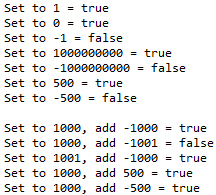
\includegraphics[scale=0.4]{test-illustrationer1.jpg}
\caption[<Text for the list of figures>]{Resultatet af testkørsel Refuge}
\label{fig:testrefuge} 
\end{figure}
\subsection{Test af Laborcamp}
\texttt{LaborCampTest} er stort set magen til. Her har vi bare trukket beløbet fra på \texttt{expected}, da vores felttype nu giver en negativ konsekvens for spilleren. Samtidig har vi omdøbt pointerne til \textit{Field}, så de hedder noget med \texttt{labor}
\subsection{Test af Tax}
Den første testklasse til \texttt{TaxTest}, er præcis magen til \texttt{LaborCampTest}. Bortset fra vi har skiftet navnene, så de passer til denne testklasse.
\subsection{Test af Tax2}
\subsection{Test af Territory}
\subsection{Test af Fleet}
\subsection{Test og fejlfinding generelt}
Vi har genbrugt vores "snydeterning" fra sidste projekt, som vi har brugt til lettere at lande på bestemte felter, når vi skulle teste en bestemt felttype.
Ellers har vi benyttet os de \textbf{White Box} tests, der var lavet en \textbf{Junit} skabelon til.